
\documentclass[12pt]{article}

\usepackage[margin=1in]{geometry}
\usepackage{graphicx}

\title{Global Impact of Sea-Level Rise}
\author{Brian Lavallee and Daniel Merrell}
\date{25 October 2019}

\begin{document}
	\maketitle

	\section{Basic Info}
		Our basic information, including emails, uIDs, and a link to the project repository, are given below.

		Brian Lavallee -- u1298898 -- brian.lavallee@utah.edu

		Daniel Merrell -- u0901346 -- daniel.r.merrell@gmail.com

		https://github.com/BrianLavallee/climate-visualization

	\section{Background and Motivation}
		We set out wanting to create some kind of visualization that had to do with the climate.
		Neither of us have background in anything climate-related, but we both think that it’s one of the most important issues the world faces today.
		Rapid climate change threatens with profound and global impacts.
		We hope to design a visualization that captures and conveys the magnitude of the potential consequences.

		In particular, we wanted to create a visualization that showed the increasing effects of climate change over time.
		Many of the datasets we explored had metrics from weather stations around the world, but we struggled to think of ways in which we could use them to tell a story about people and individuals.
		We eventually found one that has the amount of impacted landmass by country for five different sea-level rise scenarios, from 1 meter to 5 meters.
		We decided to use this data set since sea-level rise is one of the impacts of climate change that unavoidably affects large coastal regions and populations.

	\section{Project Objectives}
		We hope that the visualization will give users a better understanding of how even small increases in sea-level can impact millions of people around the world.
		Although other facets of climate change, such as severe weather events and rising temperatures, will also impact people worldwide, sea-level rise distinctly makes large areas of densely populated regions completely uninhabitable and has the potential to destroy millions of dollars of investment in those areas.
		We would like to learn specifically the amount of landmass and the number of people that will be directly impacted by various sea-level rise scenarios from mild or moderate to catastrophic.
		In an ideal situation, the visualization would be able to highlight areas with particularly dire outcomes and also show potential future timelines based on various climate forecasts.

	\section{Data}
		The main source of data is elevation maps acquired from satellite scans.
		The data comes in the form of grayscale images where the color of each pixel encodes the mean elevation of the landmass in the corresponding area.
		Each pixel represents about 64 square kilometers.
		Using this data, we will be able to determine how to draw updated world and country maps based on a given amount of sea-level rise.
		The data is available at https://www2.jpl.nasa.gov/srtm/.

		The project is mainly inspired by a sea-level rise data set that details the amount (total and percent) of impacted area in coastal countries.
		The data set only considers five scenarios from 1m to 5m.
		We hope to present this information with finer granularity in addition to visualizing the impact in geospatial form.
		We would also like to extend their data set to include information about how many people are displaced.
		However, to achieve this, we will need to acquire an additional data set on population density (mainly of coastal communities) on a similar scale to the topographic data mentioned above.
		The data set is available at https://datacatalog.worldbank.org/dataset/world-sea-level-rise-dataset.

	\section{Data Processing}
		\begin{itemize}
			\item
				Sea-Level Rise Spreadsheet

				We do not expect substantial data cleanup for this component.
				There is no missing data, and it is all well-formed.
				There are less than 100 rows of data, so it will be very easy to work with.
				If we choose to augment this data, we will mainly be working with other data sources.

			\item
				Pixel Maps

				We have obtained satellite photos of individual countries.
				The mean elevation of each grid cell is encoded by pixel brightness.
				We plan to use d3-contour to convert these pixel maps into geo-json.
				To visualize a sea-level change for a given country or region, we will re-process that region's pixel map with d3-contour at a higher threshold.
				This will effectively convert the topographic data into individual (and customizable) geo-json contours.

		\end{itemize}

	\section{Visualization Design}
		\subsection{Must-Have Features}
			\begin{itemize}
				\item
					Select a region or country and visualize the effect of rising sea-levels on the coastline.

				\item
					Select the amount sea-level rise to visualize using a slider.

				\item
					Interactive tabular view of impacted area for each sea-level rise by country.
			\end{itemize}

		\subsection{Optional Features}
			\begin{itemize}
				\item
					Draw the full world map and use zooming and panning to analyze specific regions or countries.

				\item
					Story mode that highlights areas with substantial impacts.

				\item
					Population density overlay to better encode human impact.
			\end{itemize}

	\section{Project Schedule}
		\begin{itemize}
			\item
				October 28th - November 1st:
				\begin{itemize}
					\item
						Collect all raw data

					\item
						Convert images to csv/json to be used in the visualization, requires research into data format specifics
				\end{itemize}

			\item
				November 4th - November 8th:
				\begin{itemize}
					\item
						Implement layout

					\item
						Implement tabular view and connect to header information
				\end{itemize}

			\item
				November 11th - November 15th:
				\begin{itemize}
					\item
						Implement interactivity in table including sorting and collapsing sections

					\item
						Implement slider which updates both views

					\item
						Draw regions based on sea-level rise and elevation data
				\end{itemize}

			\item
				November 18th - November 22nd:
				\begin{itemize}
					\item
						Optional feature: story mode

					\item
						Optional feature: population overlay

					\item
						Optional feature: full world-map with zoom/pan
				\end{itemize}

			\item
				November 25th - November 27th:
				\begin{itemize}
					\item
						Record narration/demo/screen-cast

					\item
						Make website available
				\end{itemize}
		\end{itemize}

	\section{Elevation Data Example}
		\vspace{-9cm}
		\includegraphics[scale=1.0]{figures/data.png}
	\section{Layout}
		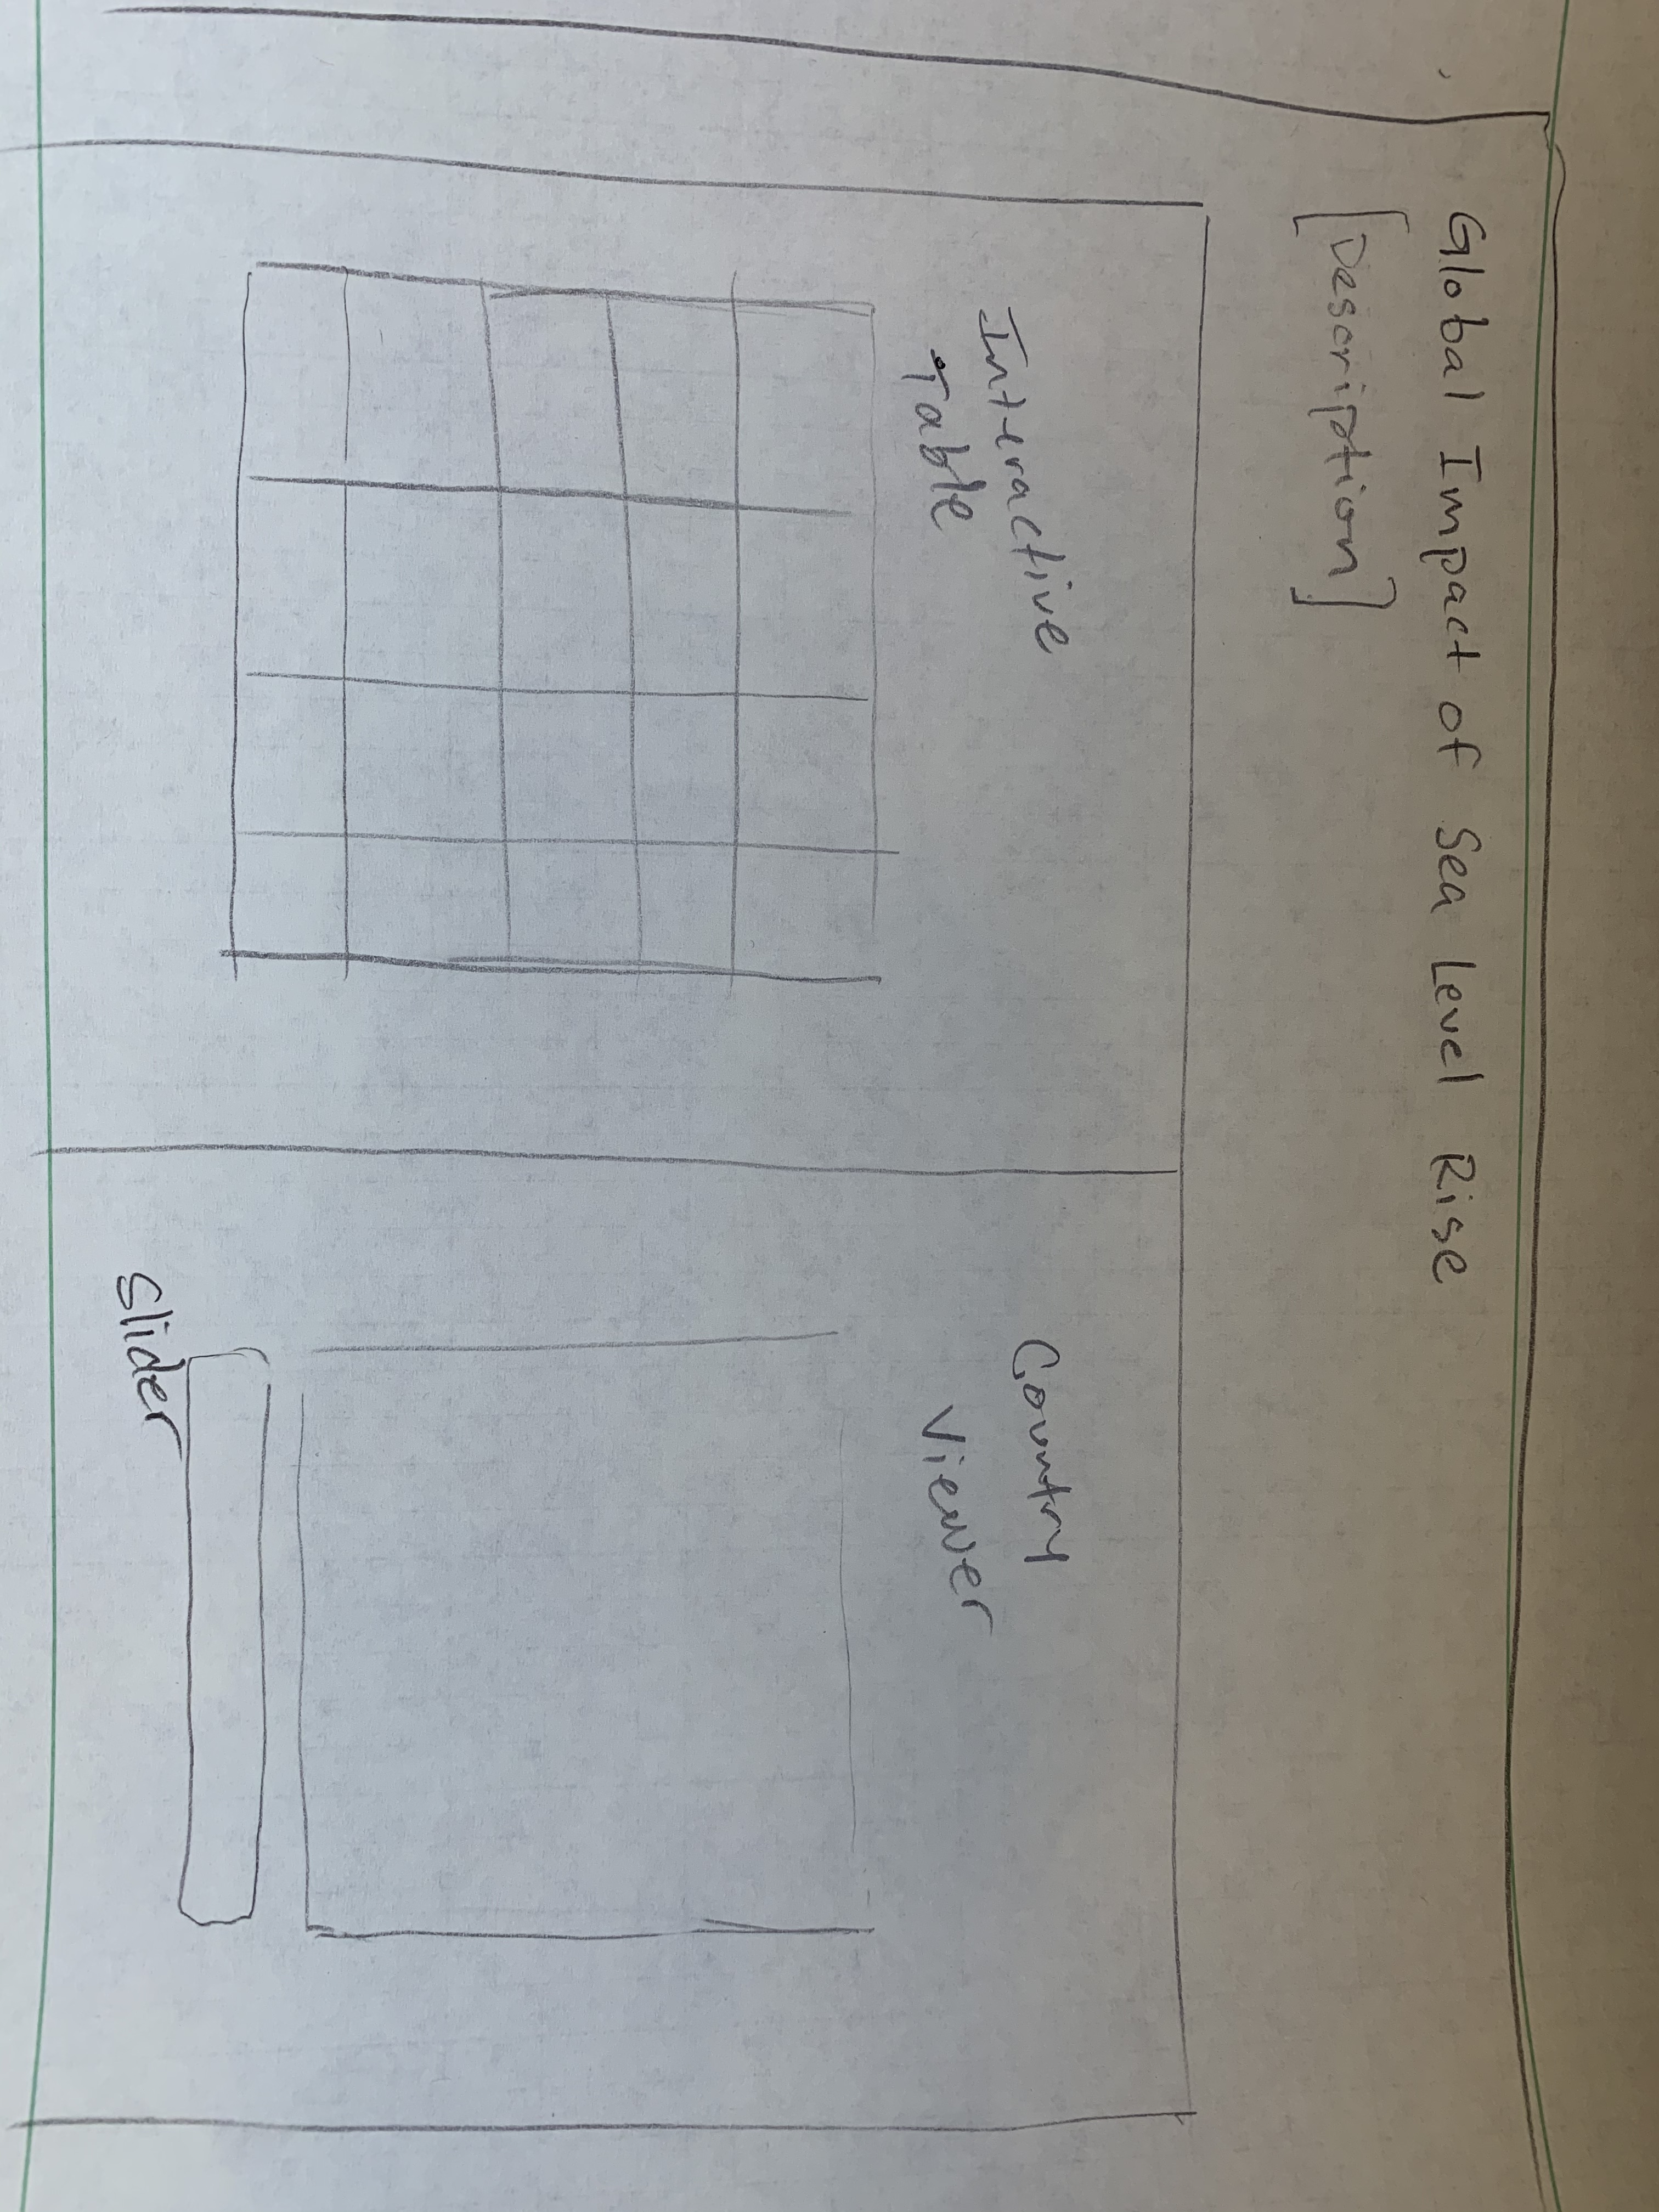
\includegraphics[scale=0.15]{figures/overview.jpg}
	\section{Tabular View}
		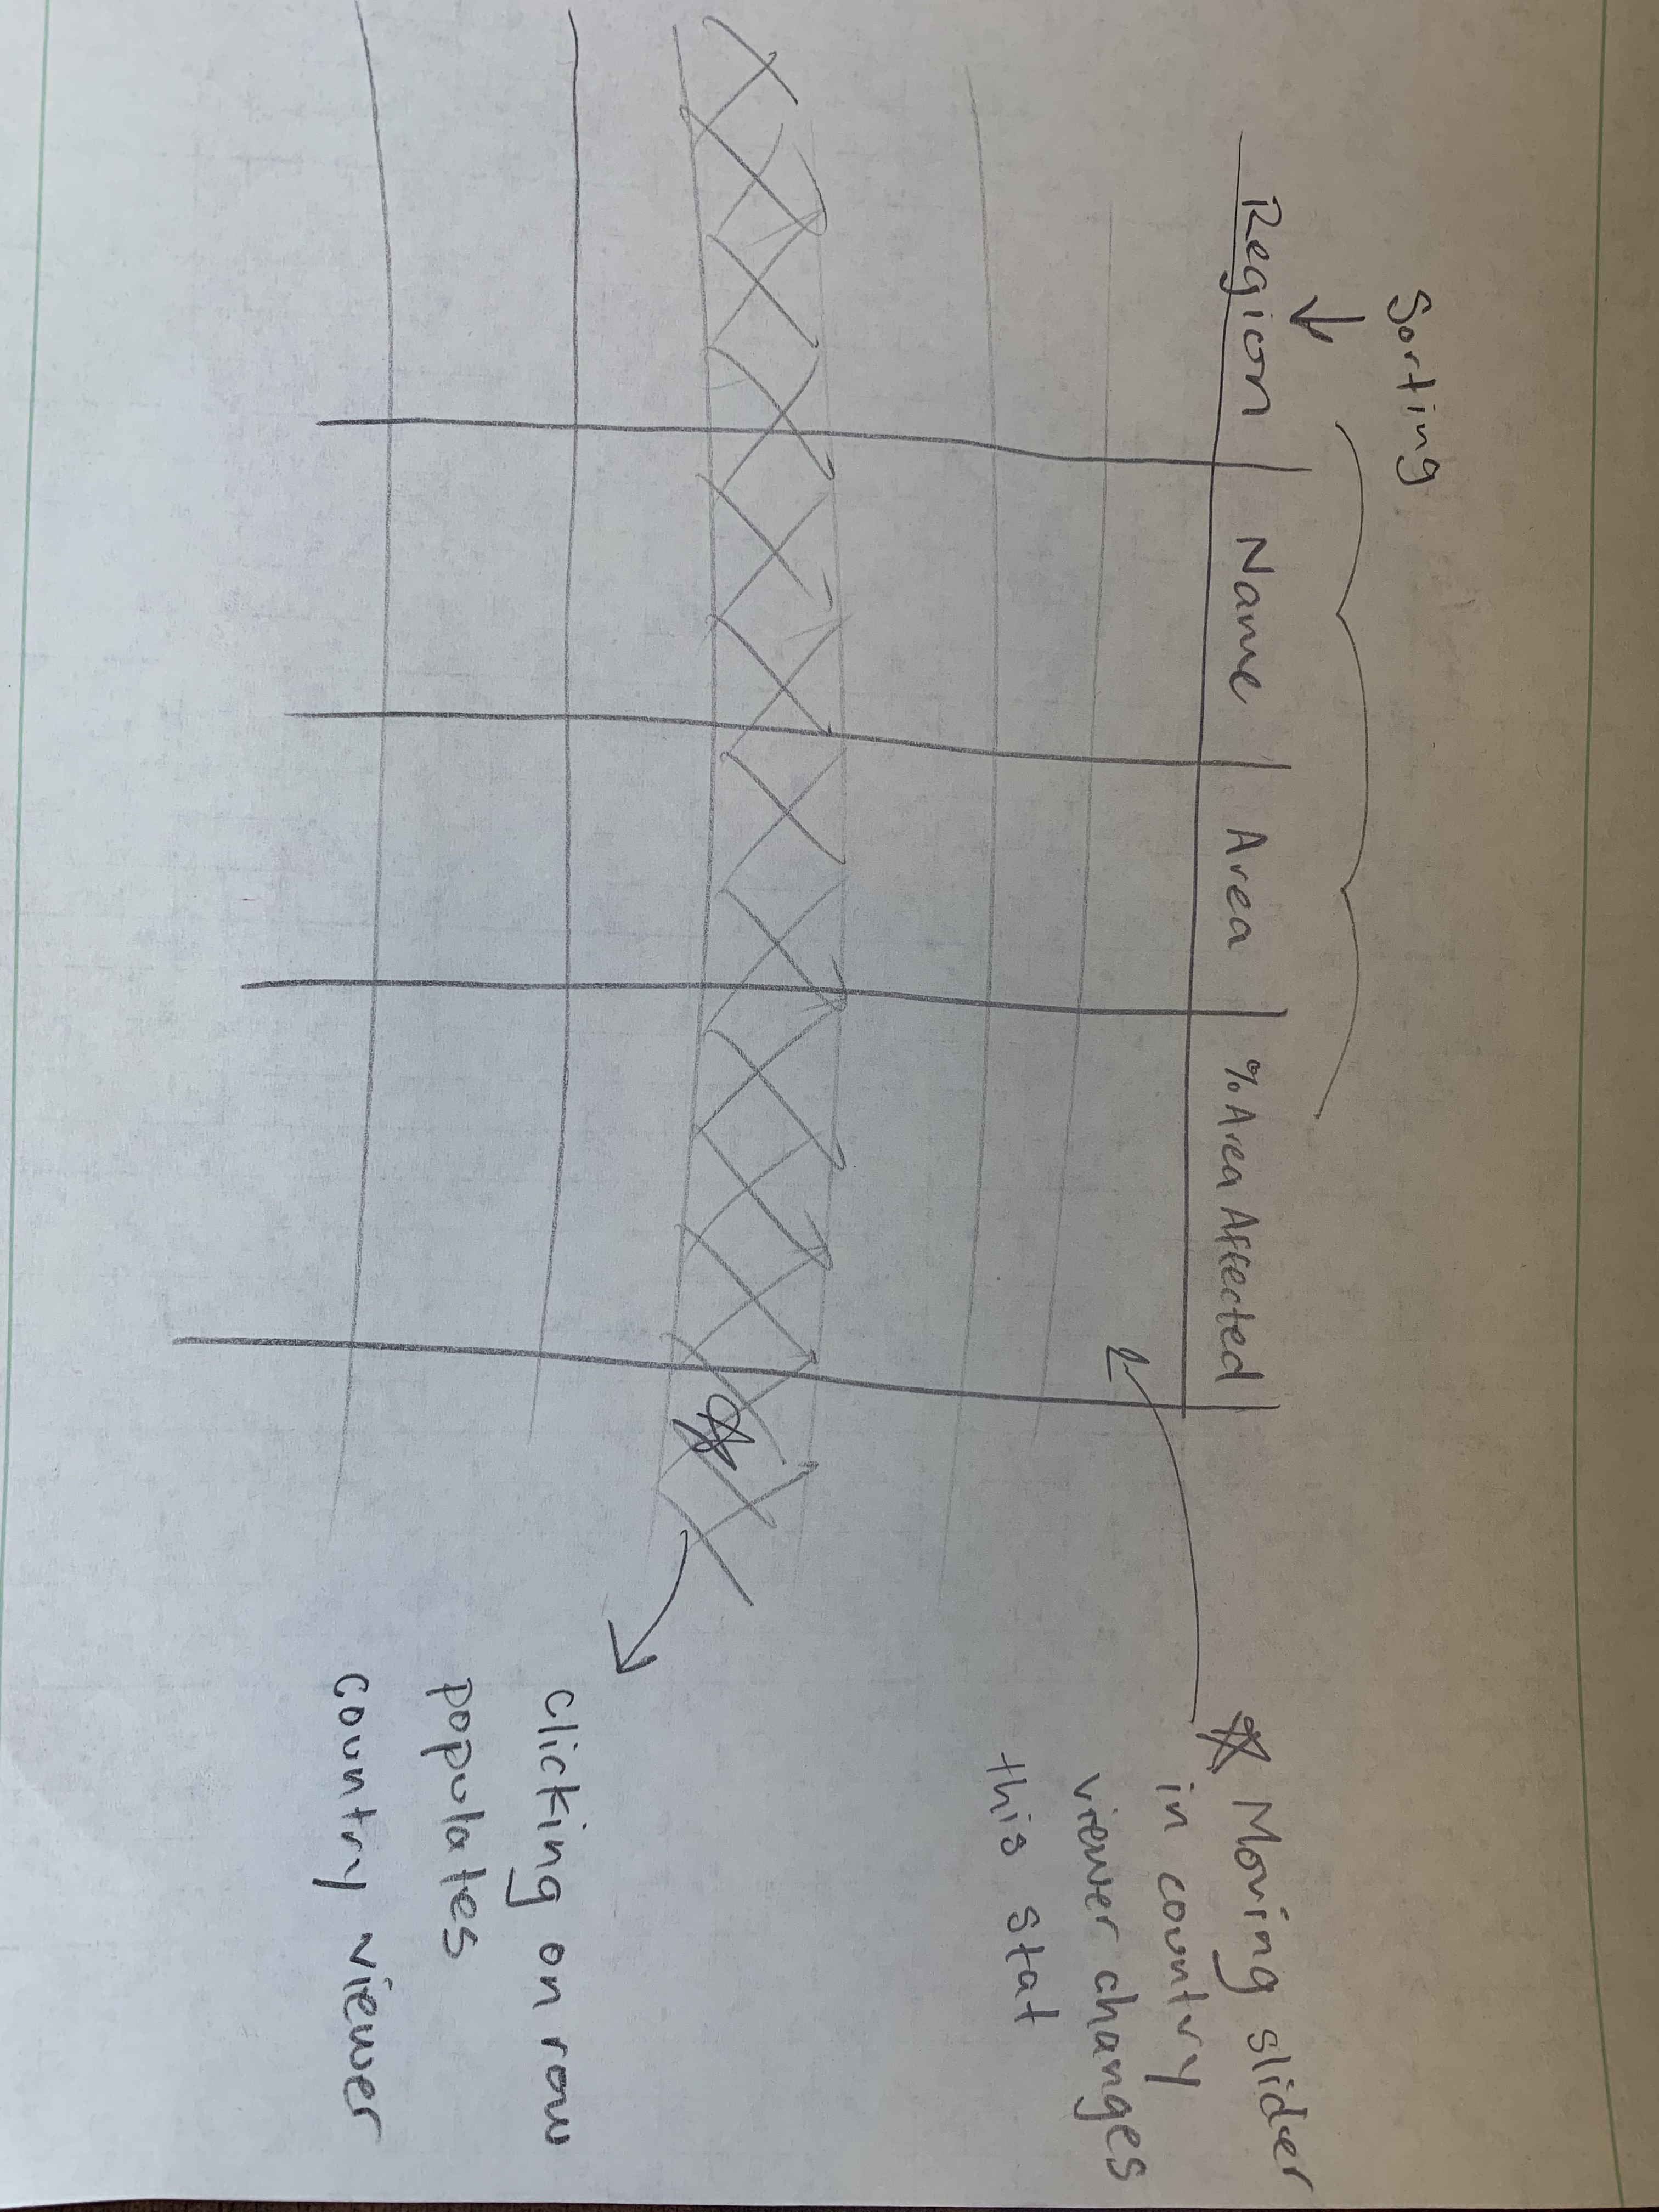
\includegraphics[scale=0.15]{figures/table-view.jpg}
	\section{Map View}
		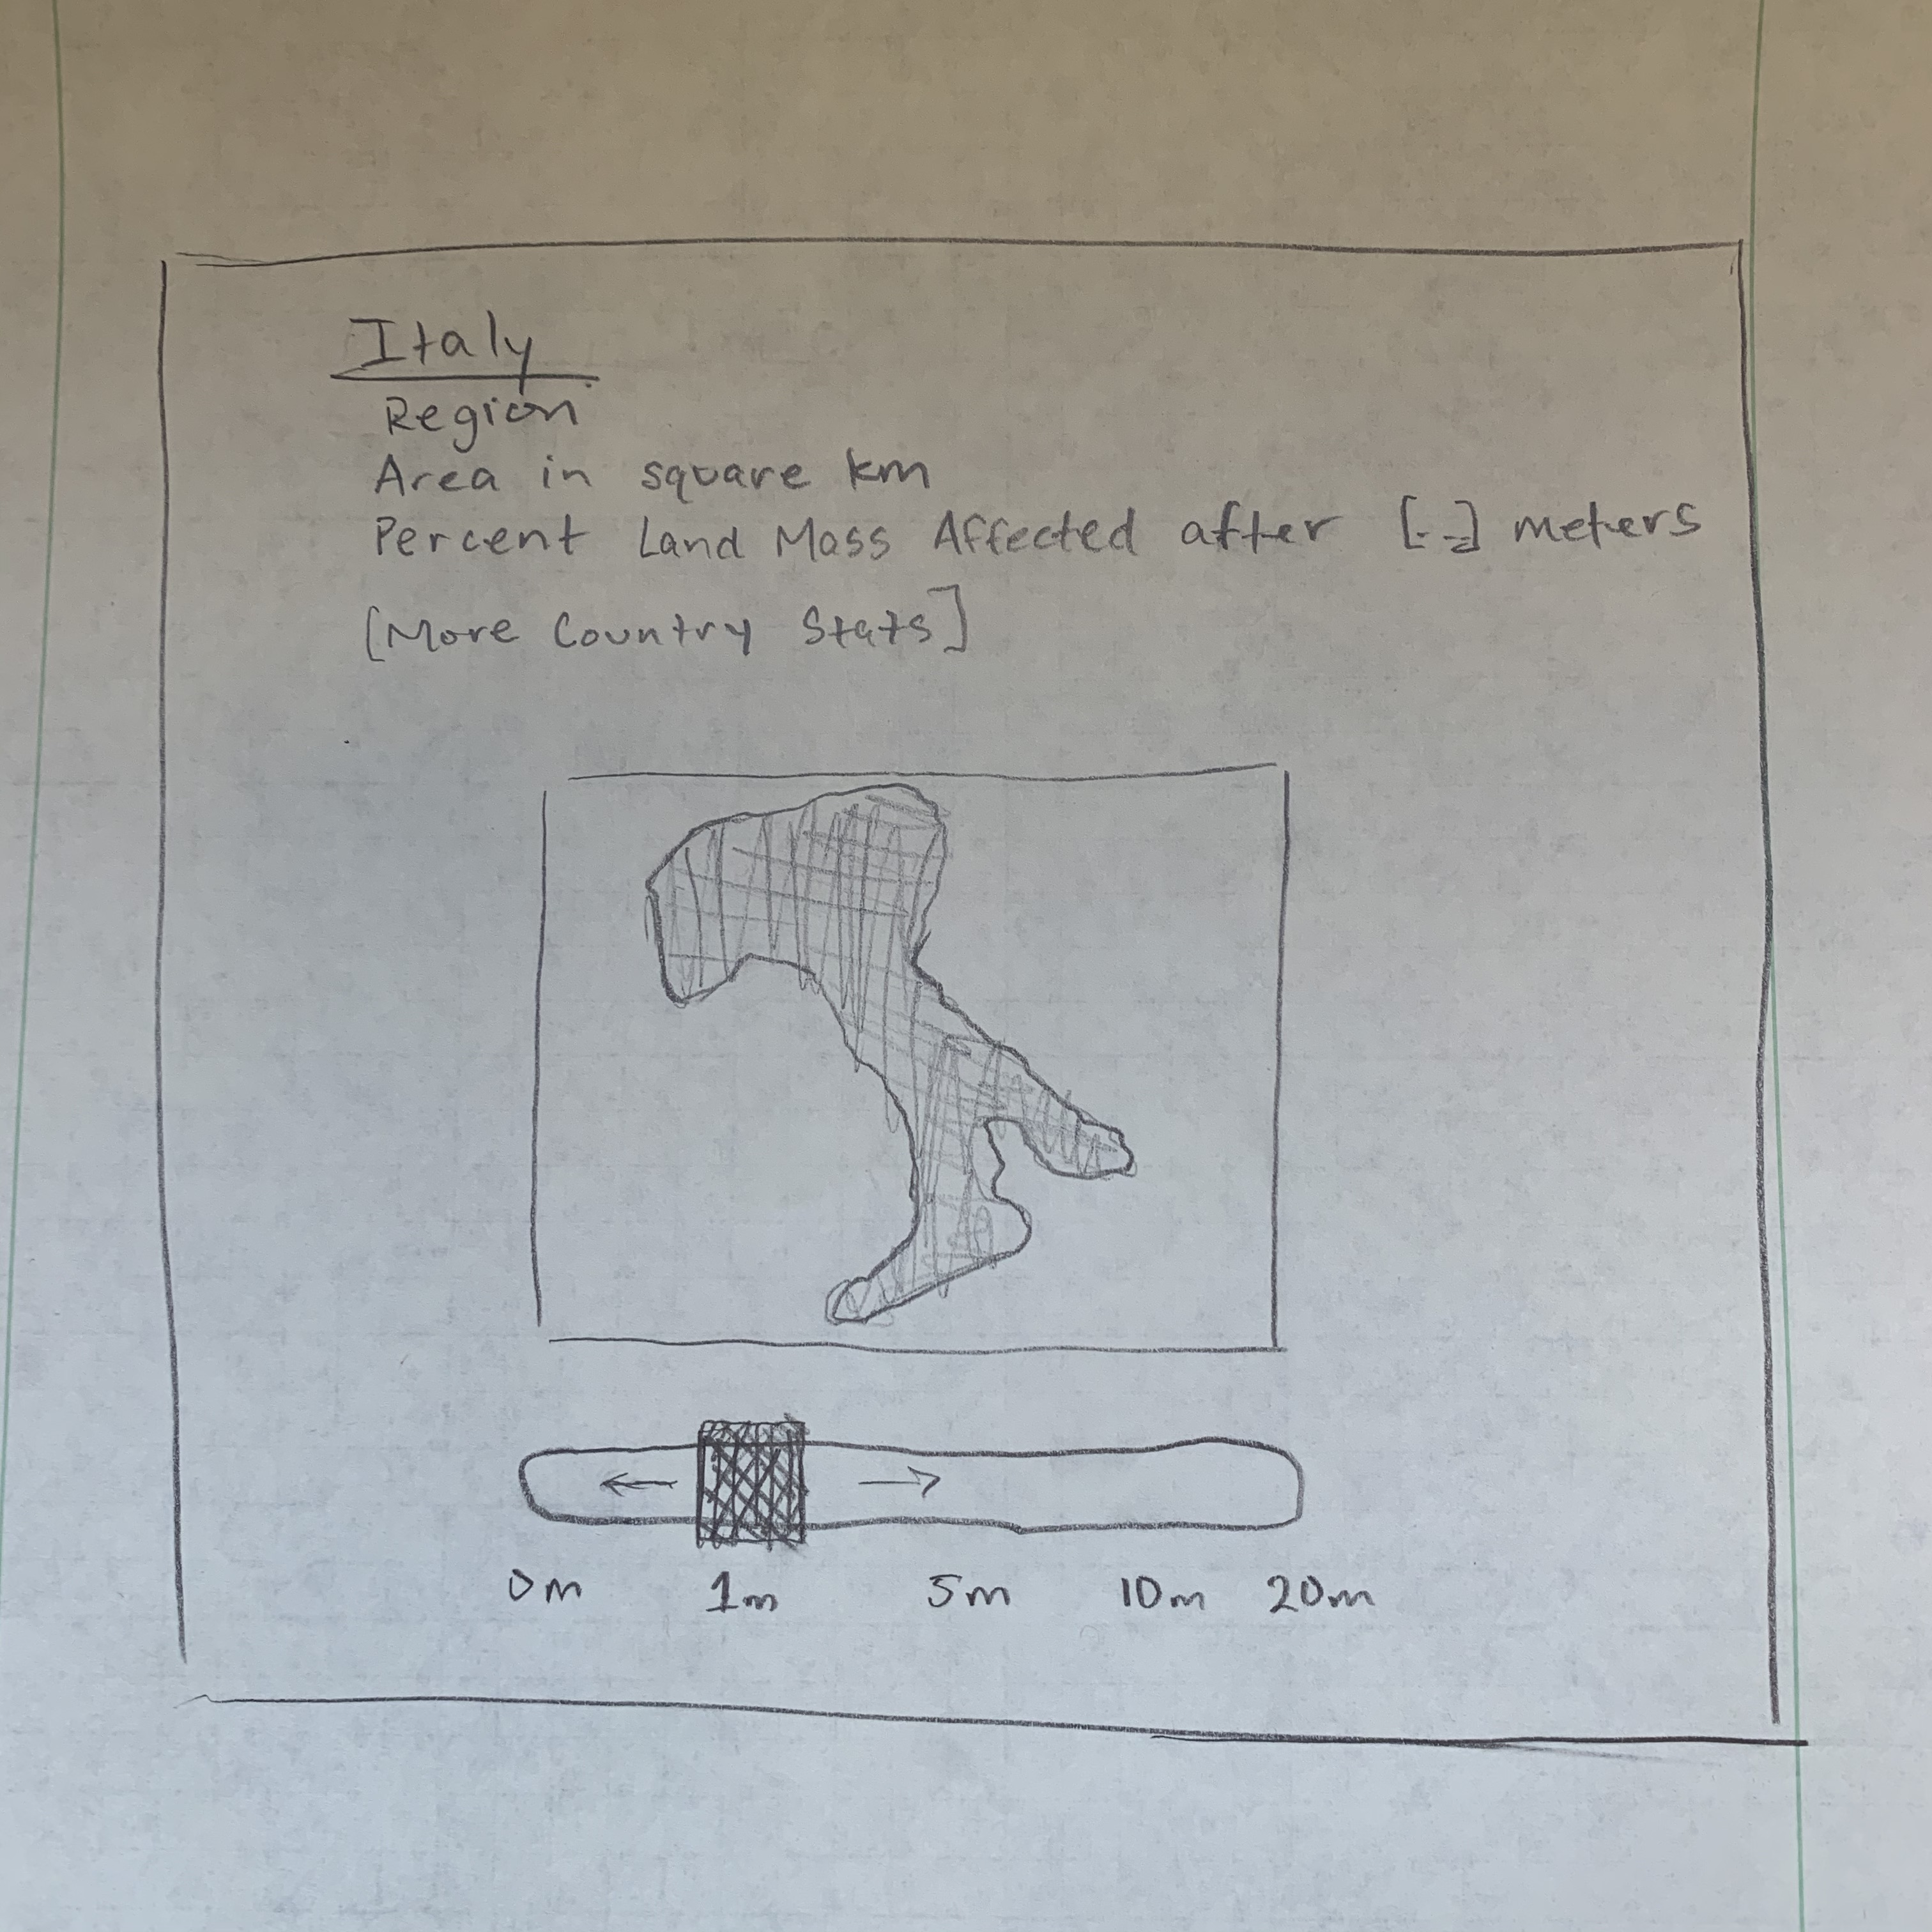
\includegraphics[scale=0.15]{figures/country-view.jpg}
\end{document}
